\chapter{Testing}

\section{Test Plan}

\begin{landscape}
\subsection{Original Outline Plan}

\begin{center}
    \begin{tabular}{|p{2cm}|p{5cm}|p{5cm}|p{4cm}|}
        \hline
        \textbf{Test Series} & \textbf{Purpose of Test Series} & \textbf{Testing Strategy} & \textbf{Strategy Rationale}\\ \hline
        1 & Test the flow of control of the user interface  & Top-Down testing &  \\ \hline
        2 & Validation of user input & Bottom-Up testing &  \\ \hline
        3 & Validation of system output & System Testing & \\ \hline
        4 & Validation of core system functionality & White box testing & \\ \hline
        5 & System performs as required by the specification & Black box testing & \\ \hline
    \end{tabular}
\end{center}

\subsection{Changes to Outline Plan}


\begin{tabular}{|l|l|}
\hline
Key: & \\ \hline
\rowcolor{DarkGray} Dark Gray & Dark grey row have been removed \\ \hline
\rowcolor{LiteGray} Lite Gray & Lite grey row have been added\\ \hline
White & Will be kept \\ \hline

\end{tabular}


\begin{center}
    \begin{tabular}{|p{2cm}|p{5cm}|p{5cm}|p{4cm}|}
        \hline
        \textbf{Test Series} & \textbf{Purpose of Test Series} & \textbf{Testing Strategy} & \textbf{Strategy Rationale}\\ \hline
        1 & Test the flow of control of the user interface  & Top-Down testing &  \\ \hline
        2 & Validation of user input & Bottom-Up testing &  \\ \hline
        3 & Validation of system output & System Testing & \\ \hline
        4 & Validation of core system functionality & White box testing & \\ \hline
        5 & System performs as required by the specification & Black box testing & \\ \hline
    \end{tabular}
\end{center}
\subsection{Original Detailed Plan}

\begin{center}
    \begin{longtable}{|p{1.5cm}|p{2.5cm}|p{2.5cm}|p{2cm}|p{2cm}|p{2cm}|p{2cm}|p{2cm}|}
        \hline
        \textbf{Test Series} & \textbf{Purpose of Test} & \textbf{Test Description} & \textbf{Test Data} & \textbf{Test Data Type (Normal/ Erroneous/ Boundary)} & \textbf{Expected Result} & \textbf{Actual Result} & \textbf{Evidence}\\ \hline
        1.01 & Test the file dialogue box & This should out put a file location and link ot the main screen & double click on file location & Normal & the database should be loaded up on the main screen &  &  \\ \hline
        
        1.02 & Testchange table buttons in the menu bar  & This should change the main layout so that it shows the table of the selected type & Click on each button in the table section of the menu bar & Normal & the main layout changes to the table of the selected type & & \\ \hline
        
        1.03 & Test the add data button for the rider table & Click on the add data button while in the club reference table & click on the add data button while in the rider table & Normal & display the add data dialogue box for the rider table & & \\ \hline
        1.04 & Test the add data button for the club reference table & Click on the add data button while in the club table & click on the add data button while in the club reference table & Normal & display the add data dialogue box for the club reference table & & \\ \hline
        1.05 & Test the add data button for the club  table & Click on the add data button while in the rider table & click on the add data button while in the club table & Normal & display the add data dialogue box for the club  table & & \\ \hline
        1.06 & Test the add data button for the record  table & Click on the add data button while in the record table & click on the add data button while in the record table & Normal & display the add data dialogue box for the record  table & & \\ \hline
        1.07 & Test the add data button for the event points  table & Click on the add data button while in the event points table & click on the add data button while in the event points table & Normal & display the add data dialogue box for the event points  table & & \\ \hline
        1.08 & Test the add data button for the event  table & Click on the add data button while in the event table & click on the add data button while in the event table & Normal & display the add data dialogue box for the event  table & & \\ \hline
        1.09 & Test the add data button for the course  table & Click on the add data button while in the course table & click on the add data button while in the course table & Normal & display the add data dialogue box for the course  table & & \\ \hline
        1.10 & Test the add data button for the event reference  table & Click on the add data button while in the event reference table & click on the add data button while in the event reference table & Normal & display the add data dialogue box for the event reference  table & & \\ \hline
        1.11 & Test the add data button for the event type  table & Click on the add data button while in the event type table & click on the add data button while in the event type table & Normal & display the add data dialogue box for the event type  table & & \\ \hline
        
        
        1.12 & Test the edit data button for the rider table & Click on the edit data button while in the club reference table & click on the edit data button while in the rider table & Normal & display the edit data dialogue box for the rider table & & \\ \hline
        1.13 & Test the edit data button for the club reference table & Click on the edit data button while in the club table & click on the edit data button while in the club reference table & Normal & display the edit data dialogue box for the club reference table & & \\ \hline
        1.14 & Test the edit data button for the club  table & Click on the edit data button while in the rider table & click on the edit data button while in the club table & Normal & display the edit data dialogue box for the club  table & & \\ \hline
        1.15 & Test the edit data button for the record  table & Click on the edit data button while in the record table & click on the edit data button while in the record table & Normal & display the edit data dialogue box for the record  table & & \\ \hline
        1.16 & Test the edit data button for the event points  table & Click on the edit data button while in the event points table & click on the edit data button while in the event points table & Normal & display the edit data dialogue box for the event points  table & & \\ \hline
        1.17 & Test the edit data button for the event  table & Click on the edit data button while in the event table & click on the edit data button while in the event table & Normal & display the edit data dialogue box for the event  table & & \\ \hline
        1.18 & Test the edit data button for the course  table & Click on the edit data button while in the course table & click on the edit data button while in the course table & Normal & display the edit data dialogue box for the course  table & & \\ \hline
        1.19 & Test the edit data button for the event reference  table & Click on the edit data button while in the event reference table & click on the edit data button while in the event reference table & Normal & display the edit data dialogue box for the event reference  table & & \\ \hline
        1.20 & Test the edit data button for the event type  table & Click on the edit data button while in the event type table & click on the edit data button while in the event type table & Normal & display the edit data dialogue box for the event type  table & & \\ \hline
        
        1.21 & Test the delete data button for the rider table & Click on the delete data button while in the club reference table & click on the delete data button while in the rider table & Normal & display the delete data dialogue box for the rider table & & \\ \hline
        1.22 & Test the delete data button for the club reference table & Click on the delete data button while in the club table & click on the delete data button while in the club reference table & Normal & display the delete data dialogue box for the club reference table & & \\ \hline
        1.23 & Test the delete data button for the club  table & Click on the delete data button while in the rider table & click on the delete data button while in the club table & Normal & display the delete data dialogue box for the club  table & & \\ \hline
        1.24 & Test the delete data button for the record  table & Click on the delete data button while in the record table & click on the delete data button while in the record table & Normal & display the delete data dialogue box for the record  table & & \\ \hline
        1.25 & Test the delete data button for the event points  table & Click on the delete data button while in the event points table & click on the delete data button while in the event points table & Normal & display the delete data dialogue box for the event points  table & & \\ \hline
        1.26 & Test the delete data button for the event  table & Click on the delete data button while in the event table & click on the delete data button while in the event table & Normal & display the delete data dialogue box for the event  table & & \\ \hline
        1.27 & Test the delete data button for the course  table & Click on the delete data button while in the course table & click on the delete data button while in the course table & Normal & display the delete data dialogue box for the course  table & & \\ \hline
        1.28 & Test the delete data button for the event reference  table & Click on the delete data button while in the event reference table & click on the delete data button while in the event reference table & Normal & display the delete data dialogue box for the event reference  table & & \\ \hline
        1.29 & Test the delete data button for the event type  table & Click on the delete data button while in the event type table & click on the delete data button while in the event type table & Normal & display the delete data dialogue box for the event type  table & & \\ \hline
        1.30 & Test the line edits of the dialogue box & Testing the line edits used in the dialogue boxes & "Peter" in the forename section of the search data for the rider table & Normal & "Peter" should be held in the line edit and can be returned & & \\ \hline
        \caption{The original test series}
        \label{tab:Original} 
    \end{longtable}
\end{center}



\subsection{Changes to Detailed Plan}

\begin{tabular}{|l|l|}
\hline
Key: & \\ \hline
\rowcolor{DarkGray} Dark Gray & Dark grey row have been removed \\ \hline
\rowcolor{LiteGray} Light Gray & Lite grey row have been added\\ \hline
White & Will be kept \\ \hline

\end{tabular}


\begin{center}
    \begin{longtable}{|p{1.5cm}|p{2.5cm}|p{2.5cm}|p{2cm}|p{2cm}|p{2cm}|p{2cm}|p{2cm}|}
        \hline
        \textbf{Test Series} & \textbf{Purpose of Test} & \textbf{Test Description} & \textbf{Test Data} & \textbf{Test Data Type (Normal/ Erroneous/ Boundary)} & \textbf{Expected Result} & \textbf{Actual Result} & \textbf{Evidence}\\ \hline
        1.01 & Test the file dialogue box & This should out put a file location and link ot the main screen & double click on file location & Normal & the database should be loaded up on the main screen & Results as expected & See figure  \ref{fig:Results of 1.01} \\ \hline
        1.02 & Test the change table buttons in the menu bar  & This should change the main layout so that it shows the table of the selected type & Click on each button in the table section of the menu bar & Normal & the main layout changes to the table of the selected type & Results as expected & \\ \hline
        1.03 & Test the add data button for the rider table & Click on the add data button while in the club reference table & click on the add data button while in the rider table & Normal & display the add data dialogue box for the rider table & Results as expected & \\ \hline
        1.04 & Test the add data button for the club reference table & Click on the add data button while in the club table & click on the add data button while in the club reference table & Normal & display the add data dialogue box for the club reference table & & \\ \hline
        1.05 & Test the add data button for the club  table & Click on the add data button while in the rider table & click on the add data button while in the club table & Normal & display the add data dialogue box for the club  table & & \\ \hline
        \rowcolor{DarkGray}1.06 & Test the add data button for the record  table & Click on the add data button while in the record table & click on the add data button while in the record table & Normal & display the add data dialogue box for the record  table & & \\ \hline
        \rowcolor{DarkGray}1.07 & Test the add data button for the event points  table & Click on the add data button while in the event points table & click on the add data button while in the event points table & Normal & display the add data dialogue box for the event points  table & & \\ \hline
        \rowcolor{DarkGray}1.08 & Test the add data button for the event  table & Click on the add data button while in the event table & click on the add data button while in the event table & Normal & display the add data dialogue box for the event  table & & \\ \hline
        \rowcolor{DarkGray}1.09 & Test the add data button for the course  table & Click on the add data button while in the course table & click on the add data button while in the course table & Normal & display the add data dialogue box for the course  table & & \\ \hline
        \rowcolor{DarkGray}1.10 & Test the add data button for the event reference  table & Click on the add data button while in the event reference table & click on the add data button while in the event reference table & Normal & display the add data dialogue box for the event reference  table & & \\ \hline
        \rowcolor{DarkGray}1.11 & Test the add data button for the event type  table & Click on the add data button while in the event type table & click on the add data button while in the event type table & Normal & display the add data dialogue box for the event type  table & & \\ \hline
        
        
        \rowcolor{DarkGray}1.12 & Test the edit data button for the rider table & Click on the edit data button while in the club reference table & click on the edit data button while in the rider table & Normal & display the edit data dialogue box for the rider table & & \\ \hline
        \rowcolor{DarkGray}1.13 & Test the edit data button for the club reference table & Click on the edit data button while in the club table & click on the edit data button while in the club reference table & Normal & display the edit data dialogue box for the club reference table & & \\ \hline
        \rowcolor{DarkGray}1.14 & Test the edit data button for the club  table & Click on the edit data button while in the rider table & click on the edit data button while in the club table & Normal & display the edit data dialogue box for the club  table & & \\ \hline
        1.15 & Test the edit data button for the record  table & Click on the edit data button while in the record table & click on the edit data button while in the record table & Normal & display the edit data dialogue box for the record  table & & \\ \hline
        1.16 & Test the edit data button for the event points  table & Click on the edit data button while in the event points table & click on the edit data button while in the event points table & Normal & display the edit data dialogue box for the event points  table & & \\ \hline
        1.17 & Test the edit data button for the event  table & Click on the edit data button while in the event table & click on the edit data button while in the event table & Normal & display the edit data dialogue box for the event  table & & \\ \hline
        \rowcolor{DarkGray}1.18 & Test the edit data button for the course  table & Click on the edit data button while in the course table & click on the edit data button while in the course table & Normal & display the edit data dialogue box for the course  table & & \\ \hline
        \rowcolor{DarkGray}1.19 & Test the edit data button for the event reference  table & Click on the edit data button while in the event reference table & click on the edit data button while in the event reference table & Normal & display the edit data dialogue box for the event reference  table & & \\ \hline
        \rowcolor{DarkGray}1.20 & Test the edit data button for the event type  table & Click on the edit data button while in the event type table & click on the edit data button while in the event type table & Normal & display the edit data dialogue box for the event type  table & & \\ \hline
        
        1.21 & Test the delete data button for the rider table & Click on the delete data button while in the club reference table & click on the delete data button while in the rider table & Normal & display the delete data dialogue box for the rider table & & \\ \hline
        1.22 & Test the delete data button for the club reference table & Click on the delete data button while in the club table & click on the delete data button while in the club reference table & Normal & display the delete data dialogue box for the club reference table & & \\ \hline
        1.23 & Test the delete data button for the club  table & Click on the delete data button while in the rider table & click on the delete data button while in the club table & Normal & display the delete data dialogue box for the club  table & & \\ \hline
        \rowcolor{DarkGray}1.24 & Test the delete data button for the record  table & Click on the delete data button while in the record table & click on the delete data button while in the record table & Normal & display the delete data dialogue box for the record  table & & \\ \hline
        \rowcolor{DarkGray}1.25 & Test the delete data button for the event points  table & Click on the delete data button while in the event points table & click on the delete data button while in the event points table & Normal & display the delete data dialogue box for the event points  table & & \\ \hline
        \rowcolor{DarkGray}1.26 & Test the delete data button for the event  table & Click on the delete data button while in the event table & click on the delete data button while in the event table & Normal & display the delete data dialogue box for the event  table & & \\ \hline
        \rowcolor{DarkGray}1.27 & Test the delete data button for the course  table & Click on the delete data button while in the course table & click on the delete data button while in the course table & Normal & display the delete data dialogue box for the course  table & & \\ \hline
        \rowcolor{DarkGray}1.28 & Test the delete data button for the event reference  table & Click on the delete data button while in the event reference table & click on the delete data button while in the event reference table & Normal & display the delete data dialogue box for the event reference  table & & \\ \hline
        \rowcolor{DarkGray}1.29 & Test the delete data button for the event type  table & Click on the delete data button while in the event type table & click on the delete data button while in the event type table & Normal & display the delete data dialogue box for the event type  table & & \\ \hline
        1.30 & Test the line edits of the dialogue box & Testing the line edits used in the dialogue boxes & "Peter" in the forename section of the search data for the rider table & Normal & "Peter" should be held in the line edit and can be returned & & \\ \hline 
        
        \rowcolor{LiteGray} 2.01 & Validate that data is being sent though the system correctly and entered in to the data base & On the event table, I will attempt to add data to the database and find whether the data has been added or not & "22/02/2015" in the date line edit,"2" in the course ID and "1" in the laps line edit then press the "ok" button & Normal & The main ui segment will be updated with the changes present  & & \\ \hline
        \rowcolor{LiteGray} 2.02 & Validate that data is being sent though the system correctly and entered in to the data base & On the rider table, I will attempt to add data to the database and find whether the data has been added or not & I will not change the default text in the add data dialogue box & Erroneous & Error box saying "All fields mush be filled" & & \\ \hline
        \rowcolor{LiteGray} 2.03 & Validate that data is being sent though the system correctly and entered in to the data base & On the rider table, I will attempt to delete data from the database and find whether the data has been deleted or not & I will change the default text in the delete data dialogue box "3" & Normal & The main ui segment will be updated with the changes present & & \\ \hline
        \rowcolor{LiteGray} 2.04 & Validate that data is being sent though the system correctly and entered in to the data base & On the course table, I will attempt to filter the data from the database and find whether the data has been filtered or not & I will not change the default text in the search data dialogue box & Erroneous & The main ui segment will be updated with no changes present & & \\ \hline
        \rowcolor{LiteGray} 2.05 & Validate that data is being sent though the system correctly and entered in to the data base & On the club table, I will attempt to filter the data from the database and find whether the data has been filtered or not & I will  change the default text in the search data dialogue box from the "Club ID" line edit to "3" & Normal & The main ui segment will be updated showing only "Cambridge Tri Club" in the club column and "3" in the ClubID column  & & \\ \hline
        
        \rowcolor{LiteGray} 3.01 & Validate that data is being out output form the system correctly by creating a new event and record for that event & On the course table I will add new data to the table using the Add Data tool bar button & I will enter "F2/10 Cam" in to the course code line edit, and "10" in to the Course Distance line edit then I will press the "ok" button & Normal & The new data will be added to the table and the main ui segment will be updated & As expected result & \\ \hline
        \rowcolor{LiteGray} 3.02 & Validate that data is being out output form the system correctly by creating a new event and records for that event & On the event table I will add new data to the table using the Add Data tool bar button  & I will enter in the Date line edit I will enter "26/02/2015", in the CourseID line edit I will enter "4" and in the Laps line edit I will enter "1" then I will press the "ok" button & Normal & The new data will be added to the table and the main ui segment will be updated & As expected, however the laps and CourseID were reversed & see figure \ref{fig:Results of 3.02} \\ \hline
        \rowcolor{LiteGray} 3.03 & Validate that data is being out output form the system correctly by creating a new event and records for that event & On the EventReference table I will add new data to the table using the Add Data tool bar button  & In the EventID line edit I will enter "9", then I shall press the "ok" button & Normal & The new data will be added to the table and the main ui segment will be updated & As expected result & \\ \hline
        \rowcolor{LiteGray} 3.04 & Validate that data is being out output form the system correctly by creating a new event and records for that event & On the EventType table I will add new data to the table using the Add Data tool bar button  & In the EventType line edit I will enter "cir", and in the EventReference line edit I will enter "7" then I shall press the "ok" button & Normal & The new data will be added to the table and the main ui segment will be updated & As Expected Result & \\ \hline
        \rowcolor{LiteGray} 3.05 & Validate that data is being out output form the system correctly by creating a new event and records for that event & On the Record table I will add new data to the table using the Add Data tool bar button  & In the RideTime line edit I will enter "00:24:43", in the Age line edit I will enter "19", in the EventID line edit I will enter "9" And in the RiderID line edit I will enter "1"  & Normal & The Record Add Data dialogue box will have all bar one line edit filled  & As Expected Result & See figure \ref{fig:Results of 3.05} \\ \hline
        \rowcolor{LiteGray} 3.06 & Validate that data is being out output form the system correctly by creating a new event and records for that event & On the Record Add Data Dialog box I will calculate the Handicap Mod & In the Add Data dialogue box I will press the Cal Handicap button and then the OK button & Normal & The Handicap Mod line edit will be filled with "00:13:20", then  the data will be added to the table and the main ui segment will be updated & The result was not as expected the "Cal Handicap" button reported an error forcing the Handicap mod not to be calculated or altered,however the record & \ref{fig:Results of 3.06} \\ \hline
        \caption{The changes to the test series}
        \label{tab:Changes} 
    \end{longtable}
\end{center}


\section{Test Data}

\subsection{Original Test Data}
The original test data can be found in table \ref{tab:Original}

\subsection{Changes to Test Data}
The original test data can be found in table \ref{tab:Changes}

\section{Annotated Samples}
\begin{figure}[H]
    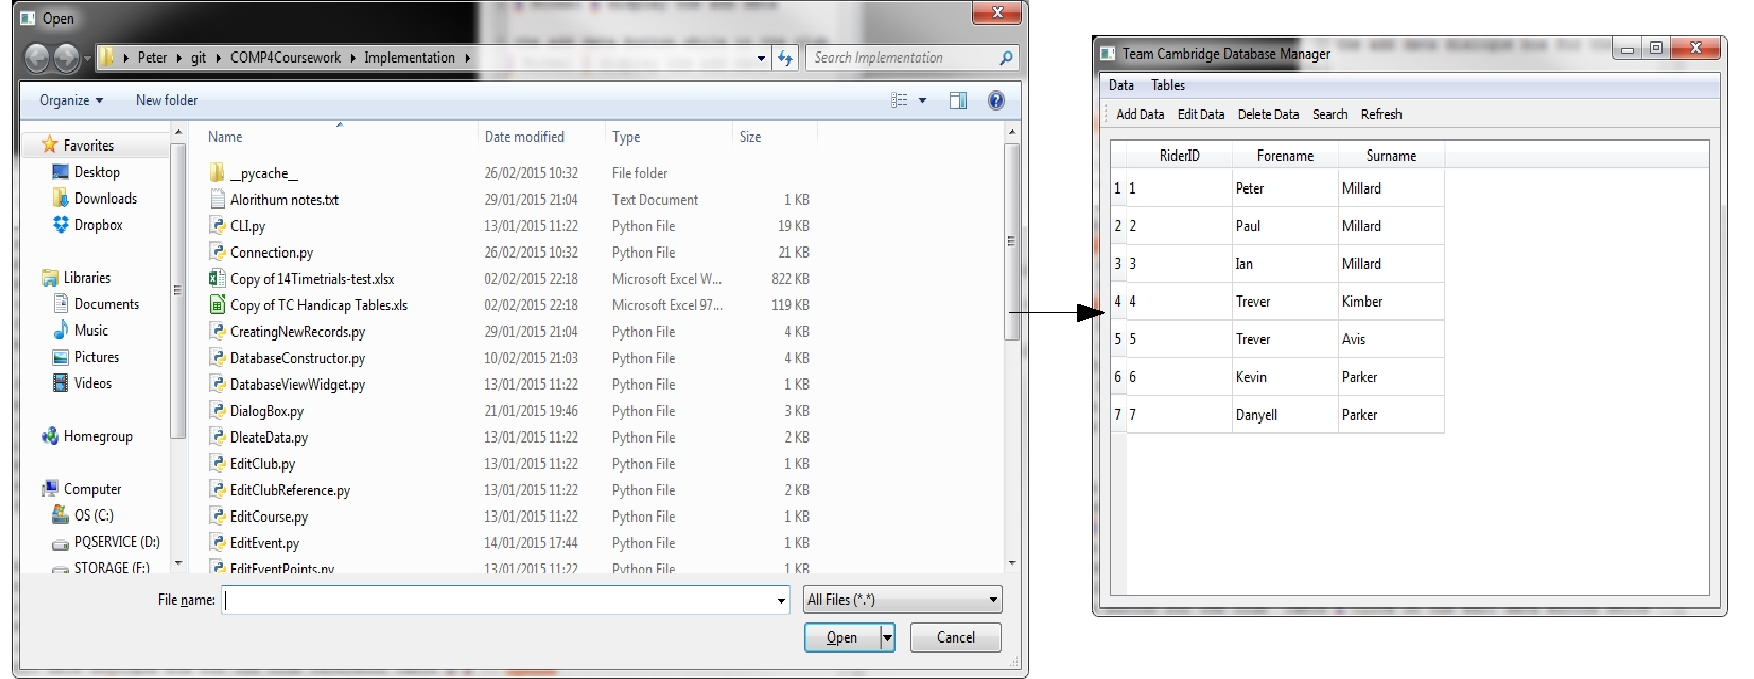
\includegraphics[width=\textwidth]{./Testing/S3/101.pdf}
    \caption{Results of 1.01} \label{fig:Results of 1.01}
\end{figure}

\begin{figure}[H]
    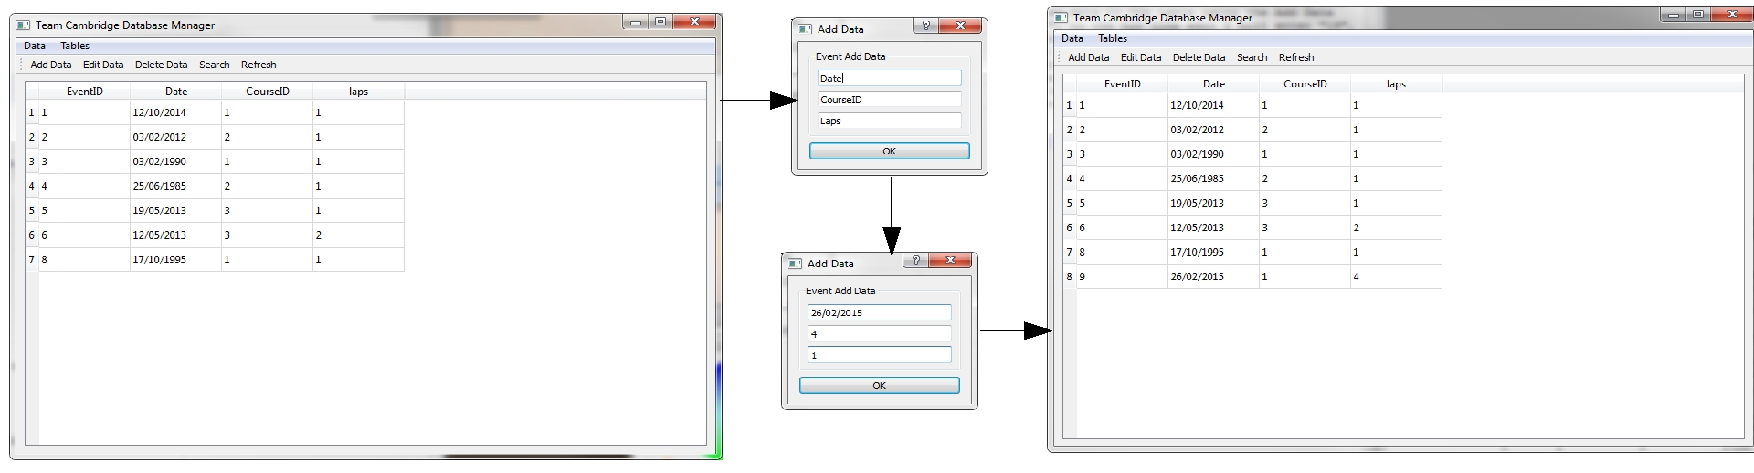
\includegraphics[width=\textwidth]{./Testing/S3/302.pdf}
    \caption{Results of 3.02} \label{fig:Results of 3.02}
\end{figure}

\begin{figure}[H]
    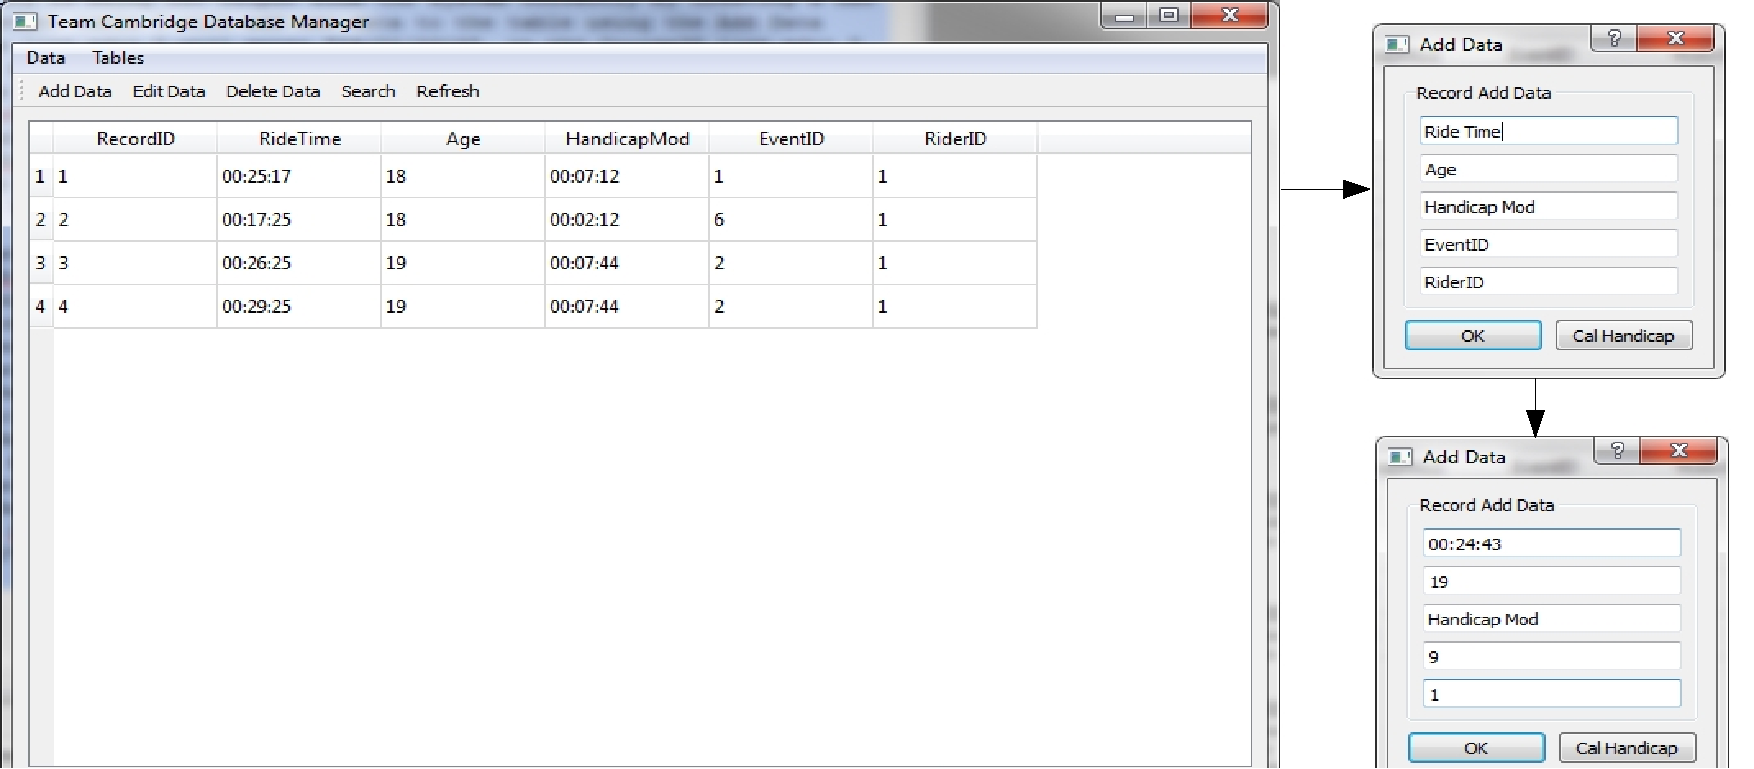
\includegraphics[width=\textwidth]{./Testing/S3/305.pdf}
    \caption{Results of 3.05} \label{fig:Results of 3.05}
\end{figure}

\begin{figure}[H]
    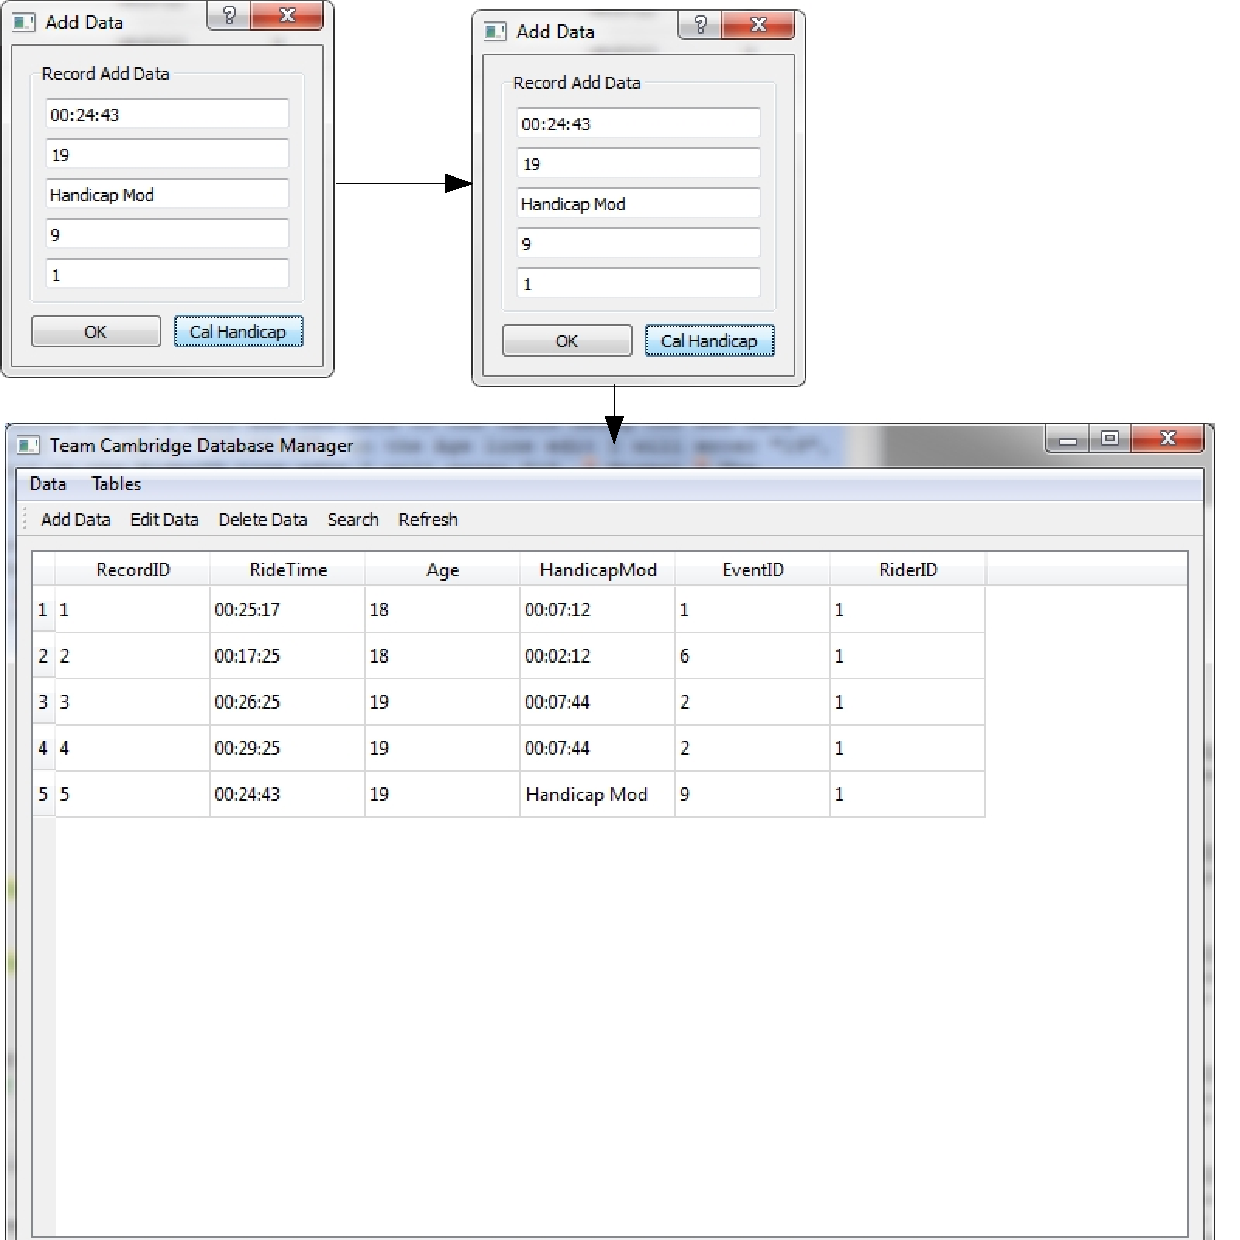
\includegraphics[width=\textwidth]{./Testing/S3/306.pdf}
    \caption{Results of 3.06} \label{fig:Results of 3.06}
\end{figure}

\subsection{Actual Results}
The Results can be found in table \ref{tab:Changes}
\subsection{Evidence}

\end{landscape}

\section{Evaluation}

\subsection{Approach to Testing}

\subsection{Problems Encountered}

\subsection{Strengths of Testing}

\subsection{Weaknesses of Testing}

\subsection{Reliability of Application}

\subsection{Robustness of Application}